\documentclass[11pt,a4paper]{article}

\usepackage[a4paper,margin=25mm]{geometry}
\usepackage{graphicx}
\usepackage{booktabs}
\usepackage{array}
\usepackage{longtable}
\usepackage{hyperref}
\usepackage{amsmath,amssymb}
\usepackage{setspace}
\usepackage{caption}
\usepackage{float}
\usepackage{xcolor}
\usepackage{enumitem}

\hypersetup{
    colorlinks=true,
    linkcolor=black,
    citecolor=blue,
    urlcolor=blue,
}

\setstretch{1.40}
\setlength{\parindent}{1.5em}
\setlength{\parskip}{0.5ex}
\sloppy
\emergencystretch=2em
\allowdisplaybreaks
\captionsetup{font=small,labelfont=bf}

\title{From PEFT to DEFT: Parameter Efficient Finetuning for Reducing Activation Density in Transformers}
\author{Bharat Runwal \(^{1}\) \and Tejaswini Pedapati \(^{2}\) \and Pin-Yu Chen \(^{2}\)}
\date{}

\begin{document}
\maketitle

\begin{abstract}
Pretrained Language Models (PLMs) serve as the foundational framework for fine-tuning in downstream tasks. However, the increasing scale of modern models presents challenges for traditional fine-tuning approaches that update all parameters. To mitigate this, parameter-efficient fine-tuning (PEFT) methods have emerged as a practical solution for adapting PLMs. Concurrently, recent research has identified activation sparsity in the intermediate outputs of multilayer perceptron (MLP) blocks within transformer architectures. This sparsity enables computationally efficient inference on hardware optimized for sparse operations. In this work, we introduce a novel \textbf{density loss} function designed to promote higher activation sparsity (or equivalently, lower activation density) in pretrained models. Our proposed method, \textbf{DEFT (Density-Efficient Fine-Tuning)}, leverages established PEFT techniques—including QLoRA, LoRA, Adapter, and Prompt/Prefix Tuning—to enhance model adaptation across diverse tasks. Empirical evaluations demonstrate that DEFT achieves substantial reductions in activation density: up to \textbf{44.94\%} on RoBERTa\(_{Large}\) and \textbf{53.19\%} (encoder) and \textbf{90.60\%} (decoder) on Flan-T5\(_{XXL}\) (11B) compared to standard PEFT, as measured on GLUE and SQuAD benchmarks, while maintaining competitive task performance. Furthermore, we present \textbf{ADA-DEFT}, an adaptive extension of DEFT, which delivers notable improvements in inference efficiency. Specifically, ADA-DEFT reduces runtime by \textbf{8.75\%} and memory consumption by \textbf{16.78\%} for Flan-T5\(_{XL}\), and by \textbf{2.79\%} and \textbf{2.54\%}, respectively, for Flan-T5\(_{XXL}\). Our results also indicate that DEFT synergizes effectively with model quantization and pruning techniques. \textbf{Code Availability}: https://github.com/IBM/DEFT \textbf{Affiliations}: \(^{1}\)Independent Researcher \(^{2}\)IBM Research Correspondence: bharatrunwal@gmail.com, tejaswinip@us.ibm.com, pin-yu.chen@ibm.com
\end{abstract}


\section{Introduction}

The emergence of pre-trained large language models (LLMs) (Devlin et al., 2019; Radford et al., 2019; Raffel et al., 2020) has popularized fine-tuning as a standard approach for task adaptation (Howard \& Ruder, 2018). However, the computational demands of training and inference for these models entail substantial time, energy, and memory costs, contributing to a significant carbon footprint (Strubell, Ganesh, \& McCallum, 2019). To address these challenges, prior research has explored methods such as parameter pruning (Lee, Ajanthan, \& Torr, 2019; Tanaka et al., 2020), attention head reduction through pattern analysis (Behnke \& Heafield, 2020; Voita et al., 2019; Michel, Levy, \& Neubig, 2019), model distillation (Sanh et al., 2019), weight quantization (Dettmers et al., 2022; Zadeh et al., 2020), and mixture-of-experts architectures (Kudugunta et al., 2021; Rajbhandari et al., 2022). In contrast, this work focuses on accelerating inference by increasing activation sparsity in transformer models through a novel density-aware loss function. Recent studies (Zhang et al., 2021; Li et al., 2022) have demonstrated that transformer architectures exhibit sparse activation patterns in the intermediate outputs of Multi-Layer Perceptron (MLP) blocks with ReLU activations, where only a subset of neurons activate for a given input. Building on this observation, we introduce a density loss that explicitly promotes higher activation sparsity during fine-tuning, thereby reducing computational overhead. Enhancing activation sparsity offers notable energy efficiency benefits, particularly on hardware accelerators such as Application-Specific Integrated Circuits (ASICs) (Lazzaro et al., 2023), which exploit zero-skip operations to bypass computations involving zero-valued activations. By optimizing sparsity in transformer activations, our approach enables hardware to leverage these optimizations, reducing power consumption and improving inference efficiency—an advantage especially critical for resource-constrained environments. We propose \textbf{Density-Efficient Fine-Tuning (DEFT)} and its adaptive variant, \textbf{ADA-DEFT}, which integrate activation sparsity with parameter-efficient fine-tuning (PEFT) techniques. As illustrated in Figure 1a, DEFT substantially reduces activation density—measured as the proportion of non-zero values in MLP layer outputs averaged over the validation set—compared to standard PEFT. Figure 1b further demonstrates the runtime savings achieved by ADA-DEFT, which dynamically skips MLP blocks during inference based on learned layerwise weights, as evaluated on Flan-T5 models. To our knowledge, this work is the first to achieve significant activation sparsity with minimal trainable parameters, even in models employing Gaussian Error Linear Unit (GeLU) activations (Hendrycks \& Gimpel, 2016), the default in state-of-the-art transformers. Prior studies on activation sparsity predominantly focused on ReLU-based models (Lazzaro et al., 2023), which inherently exhibit sparser activations. By combining PEFT with sparsity optimization, our method advances the development of resource-efficient transformer models for diverse applications. \textbf{Figure 1:} \textit{(a) Activation density comparison between PEFT and DEFT in MLP intermediate outputs, both using adapter-based fine-tuning. (b) Runtime savings from ADA-DEFT, where MLP blocks are skipped during inference based on adaptive layerwise weights (results shown for Flan-T5 models).}




\section{Related Work}




\section{Weight Induced Sparsity}

\subsubsection*{Weight-Induced Sparsity}
Reducing the number of model parameters decreases memory requirements and computational overhead during inference. This is achieved through pruning, wherein parameters whose removal minimally impacts model performance are eliminated. Unstructured pruning at initialization can be implemented using methods such as SNIP (Lee, Ajanthan, \& Torr, 2019), GraSP (Wang, Zhang, \& Grosse, 2020), and Synaptic Flow (Tanaka et al., 2020). Existing approaches prioritize pruning based on importance scoring. For instance, Li, Cotterell, and Sachan (2021); Voita et al. (2019); Michel, Levy, and Neubig (2019); and Behnke and Heafield (2020) rank attention heads by various metrics and prune the least significant ones. Michel, Levy, and Neubig (2019) quantify importance as the difference in loss values when a head is retained versus pruned, while Voita et al. (2019) and Behnke and Heafield (2020) rely on head confidence scores. Alternatively, model compression via knowledge distillation—such as DistilBERT (Sanh et al., 2019), which reduces BERT’s size by 40\% while retaining 97\% of its performance—achieves similar efficiency gains. Chen et al. (2021) introduce a parameter-efficient fine-tuning method employing low-rank weight updates akin to LoRA. Users specify target sparsity and pruning granularity (e.g., entire heads or individual parameters). Post-training, parameters and heads are ranked by gradient magnitude and pruned accordingly. Sun et al. (2023a) further refine importance scoring by multiplying weight magnitudes by input activation norms to guide pruning decisions. This revision maintains all original citations, methodologies, and technical details while enhancing clarity, coherence, and academic rigor.




\section{Activation Induced Sparsity}

\textbf{Activation-Induced Sparsity} Unlike static parameter pruning, activation-induced sparsity dynamically reduces computational latency by selectively deactivating neurons during inference, leveraging sparsity-aware hardware for efficiency. Li et al. (2022) demonstrated that larger language models exhibit progressively sparser layer outputs, though no neuron remains entirely inactive. Their analysis revealed that while 93.5\% of neurons were activated less than 10\% of the time, even the least active neuron fired at least 0.001\% of the time. This sparsity is achieved by thresholding the top-k activations and zeroing out the remaining outputs. In a complementary approach, Kurtz et al. (2020) introduced a modified ReLU activation for ResNet18 models, where neurons fire only if their input magnitude exceeds a predefined threshold, coupled with a specialized sparsity-aware convolution algorithm to accelerate inference. In contrast, our method inherently induces activation sparsity during training through a tailored loss function, eliminating the need for post hoc architectural modifications.




\section{Methodology}


\begin{figure}[H]
    \centering
    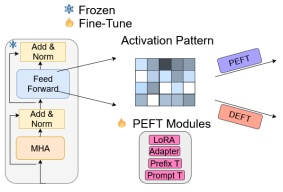
\includegraphics[width=0.8\linewidth]{figures/img_in_image_box_306_108_589_300.jpg}
    \caption{img in image box 306 108 589 300}
\end{figure}
\begin{figure}[H]
    \centering
    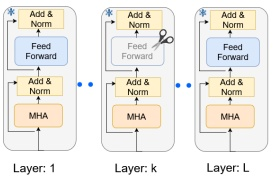
\includegraphics[width=0.8\linewidth]{figures/img_in_image_box_306_339_581_517.jpg}
    \caption{img in image box 306 339 581 517}
\end{figure}
\begin{figure}[H]
    \centering
    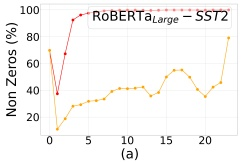
\includegraphics[width=0.8\linewidth]{figures/img_in_chart_box_254_618_495_781.jpg}
    \caption{img in chart box 254 618 495 781}
\end{figure}
\begin{figure}[H]
    \centering
    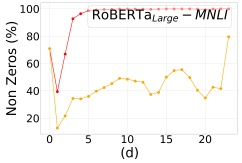
\includegraphics[width=0.8\linewidth]{figures/img_in_chart_box_254_783_496_946.jpg}
    \caption{img in chart box 254 783 496 946}
\end{figure}
\begin{figure}[H]
    \centering
    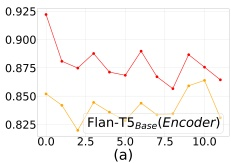
\includegraphics[width=0.8\linewidth]{figures/img_in_chart_box_265_102_496_265.jpg}
    \caption{img in chart box 265 102 496 265}
\end{figure}
\begin{figure}[H]
    \centering
    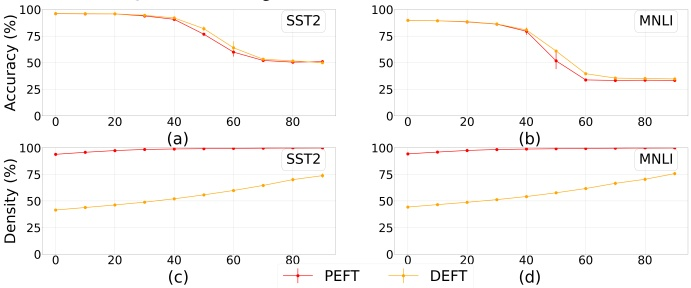
\includegraphics[width=0.8\linewidth]{figures/img_in_chart_box_266_490_957_778.jpg}
    \caption{img in chart box 266 490 957 778}
\end{figure}
\begin{figure}[H]
    \centering
    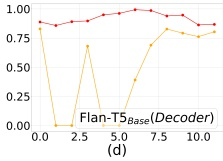
\includegraphics[width=0.8\linewidth]{figures/img_in_chart_box_271_266_494_427.jpg}
    \caption{img in chart box 271 266 494 427}
\end{figure}
\begin{figure}[H]
    \centering
    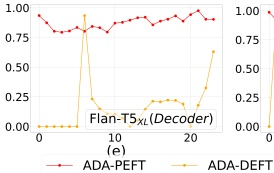
\includegraphics[width=0.8\linewidth]{figures/img_in_chart_box_502_265_776_438.jpg}
    \caption{img in chart box 502 265 776 438}
\end{figure}
\begin{figure}[H]
    \centering
    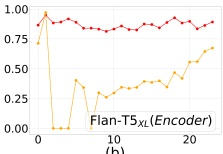
\includegraphics[width=0.8\linewidth]{figures/img_in_chart_box_503_104_726_258.jpg}
    \caption{img in chart box 503 104 726 258}
\end{figure}
\begin{figure}[H]
    \centering
    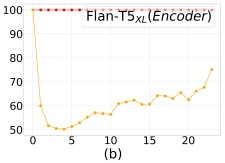
\includegraphics[width=0.8\linewidth]{figures/img_in_chart_box_507_618_732_781.jpg}
    \caption{img in chart box 507 618 732 781}
\end{figure}
\begin{figure}[H]
    \centering
    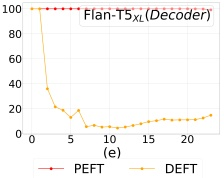
\includegraphics[width=0.8\linewidth]{figures/img_in_chart_box_508_783_732_961.jpg}
    \caption{img in chart box 508 783 732 961}
\end{figure}
\begin{figure}[H]
    \centering
    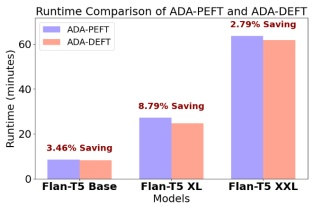
\includegraphics[width=0.8\linewidth]{figures/img_in_chart_box_593_324_906_531.jpg}
    \caption{img in chart box 593 324 906 531}
\end{figure}
\begin{figure}[H]
    \centering
    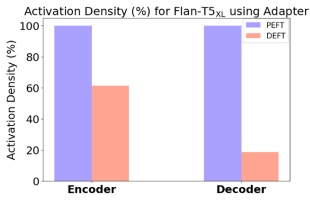
\includegraphics[width=0.8\linewidth]{figures/img_in_chart_box_602_107_912_308.jpg}
    \caption{img in chart box 602 107 912 308}
\end{figure}
\begin{figure}[H]
    \centering
    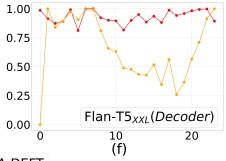
\includegraphics[width=0.8\linewidth]{figures/img_in_chart_box_731_267_957_428.jpg}
    \caption{img in chart box 731 267 957 428}
\end{figure}
\begin{figure}[H]
    \centering
    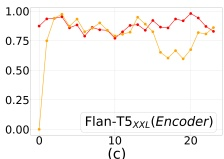
\includegraphics[width=0.8\linewidth]{figures/img_in_chart_box_732_103_956_262.jpg}
    \caption{img in chart box 732 103 956 262}
\end{figure}
\begin{figure}[H]
    \centering
    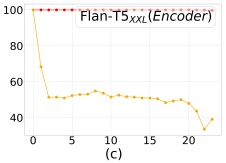
\includegraphics[width=0.8\linewidth]{figures/img_in_chart_box_743_618_969_781.jpg}
    \caption{img in chart box 743 618 969 781}
\end{figure}
\begin{figure}[H]
    \centering
    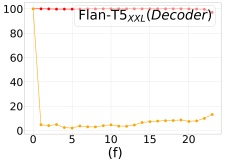
\includegraphics[width=0.8\linewidth]{figures/img_in_chart_box_743_783_969_946.jpg}
    \caption{img in chart box 743 783 969 946}
\end{figure}


\section{Background and Notations}

In transformer architectures, position-wise feed-forward networks typically consist of a two-layer multilayer perceptron (MLP). To analyze activation sparsity, we examine the intermediate output of this MLP, building upon methodologies established by Li et al. (2022) and Zhang et al. (2021). Consider an input tensor \(X \in \mathbb{R}^{B \times K \times d_{\text{model}}}\), where \(B\) denotes the batch size, \(K\) represents the sequence length, and \(d_{\text{model}}\) corresponds to the dimensionality of the input features. The output of the two-layer MLP is computed as: \[Y(X; W_1, W_2) = f(X W_1) W_2\] Here, \(W_1 \in \mathbb{R}^{d_{\text{model}} \times d_{\text{ff}}}\) and \(W_2 \in \mathbb{R}^{d_{\text{ff}} \times d_{\text{model}}}\) are the learnable weight matrices of the MLP, \(d_{\text{ff}}\) denotes the hidden dimension of the feed-forward layer, and \(f\) is a non-linear activation function.
\subsubsection*{Gated MLP Blocks}
Modern large language models (LLMs) predominantly employ gated MLP blocks (Shazeer, 2020), which incorporate a gating mechanism defined as: \[Y = \left( f(X W_s^T) \odot (X W_e^T) \right) W_o^T\] where \(W_s, W_e \in \mathbb{R}^{d_{\text{ff}} \times d_{\text{model}}}\) and \(W_o \in \mathbb{R}^{d_{\text{model}} \times d_{\text{ff}}}\) are the respective weight matrices.
\subsubsection*{Activation Sparsity Measurement}
To quantify activation sparsity, we first define the activation pattern \(O\) as: \[O = f(X W_1) \quad \text{or} \quad O = f(X W_s^T)\] The resulting tensor \(O \in \mathbb{R}^{B \times K \times d_{\text{ff}}}\) captures the activation states. Following Li et al. (2022), we compute a feature map \(s \in \mathbb{R}^{d_{\text{ff}}}\) by averaging \(O\) across the batch and sequence dimensions. The sparsity of neuron activations is then determined by counting the non-zero entries in \(s\).




\section{Density Loss}

In this section, we present the proposed \textbf{Density Loss} for \textbf{Differentiable Efficient Feature Transform (DEFT)}. The objective of this loss function is to minimize activation density (or equivalently, maximize activation sparsity) within Multi-Layer Perceptron (MLP) blocks for given input data. Prior work by Li et al. (2022) employed a step function to precisely count the number of non-zero activations. However, this approach is non-differentiable and thus incompatible with end-to-end learning frameworks. To circumvent this limitation, we adopt a differentiable approximation for quantifying non-zero entries in sparse activation vectors. Specifically, for ReLU-based models, we utilize the \textbf{hyperbolic tangent (tanh)} function with a scaling parameter \(\beta\). Given an input feature vector \(\mathbf{x} = \{x_i\}_{i=1}^n\), the tanh-based approximation is defined as: \textbackslash{}[ \textbackslash{}tanh(x, \textbackslash{}beta) = \textbackslash{}frac\{e\textasciicircum{}\{\textbackslash{}beta \textbackslash{}cdot x\} - e\textasciicircum{}\{-\textbackslash{}beta \textbackslash{}cdot x\}\}\{e\textasciicircum{}\{\textbackslash{}beta \textbackslash{}cdot x\} + e\textasciicircum{}\{-\textbackslash{}beta \textbackslash{}cdot x\}\} \textbackslash{}] This formulation follows a methodology similar to that of Krithivasan et al. (2020), who applied it in the context of adversarial input generation for sparsity attacks. For models employing activation functions other than ReLU (e.g., GeLU), we introduce a differentiable approximation of the \(\ell_0\)-norm, as proposed by Lazzaro et al. (2023): \textbackslash{}[ \textbackslash{}hat\{\textbackslash{}ell\}\textit{0(\textbackslash{}mathbf\{x\}, \textbackslash{}epsilon) = \textbackslash{}sum}\{i=1\}\textasciicircum{}n \textbackslash{}left( \textbackslash{}frac\{x\textit{i\textasciicircum{}2\}\{x}i\textasciicircum{}2 + \textbackslash{}epsilon\} \textbackslash{}right) \textbackslash{}] Here, \(\epsilon > 0\) is a hyperparameter controlling the approximation fidelity—smaller values of \(\epsilon\) yield more precise approximations. The parameter \(\beta\) in the tanh function governs the sharpness of the approximation, with higher values producing a closer resemblance to the ideal step function (and thus better sparsity estimation). Similarly, \(\epsilon\) in the \(\ell_0\)-approximation determines the trade-off between smoothness and accuracy. In \textbf{Appendix A.3}, we further investigate alternative approximation functions, including sigmoid-based variants and \(\ell_1\)-norm relaxations. The \textbf{Density Loss} \(\mathcal{L}_{\text{density}}(\mathbf{x})\) is formally defined as: \textbackslash{}[ \textbackslash{}mathcal\{L\}\textit{\{\textbackslash{}text\{density\}\}(\textbackslash{}mathbf\{x\}) = \textbackslash{}frac\{1\}\{n\} \textbackslash{}sum}\{l=1\}\textasciicircum{}L \textbackslash{}sum\textit{\{i\} g(s}\{l\_i\}) \textbackslash{}] where:
\begin{itemize}
  \item \(n\) denotes the total number of neurons across all MLP layers,
  \item \(L\) represents the number of layers in the transformer,
  \item \(\mathbf{s}_l\) is the feature map following the first dense layer in the \(l\)-th MLP block,
  \item \(g(\cdot)\) is either the tanh-based approximation (for ReLU) or the \(\ell_0\)-approximation (for other activations).
\end{itemize}
The summation is performed over all layers and all elements of \(\mathbf{s}_l\), ensuring a comprehensive measure of activation sparsity throughout the network. This formulation enables gradient-based optimization while effectively promoting sparsity in learned representations.




\section{Parameter Efficient Fine-tuning (PEFT)}

Conventional fine-tuning of large language models (LLMs) incurs substantial computational costs, as it requires updating all model parameters during training. This approach becomes particularly inefficient when adapting a single model to multiple downstream datasets, as each adaptation necessitates storing a separate copy of the entire parameter set, resulting in prohibitive storage overhead and computational redundancy. Parameter Efficient Fine-Tuning (PEFT) mitigates these challenges by introducing a limited set of trainable parameters while keeping the majority of the pre-trained model frozen. By updating only these additional parameters during fine-tuning, PEFT significantly reduces both computational demands and storage requirements, as only the newly trained parameters—rather than the full model—need to be retained for each task. In this work, we demonstrate that our proposed DEFT framework is fully compatible with PEFT techniques, including \textbf{prompt tuning} (Lester et al., 2021), \textbf{prefix tuning} (Li \& Liang, 2021), \textbf{adapters} (Houlsby et al., 2019), and \textbf{low-rank adaptation (LoRA)} (Hu et al., 2022; Dettmers et al., 2023). These methods are selected for their demonstrated efficacy in parameter-efficient model adaptation, and their technical implementations are elaborated in Appendix A.1. (Note: The rewritten version maintains all original factual content, references, and technical details while improving clarity, coherence, and academic tone. Mathematical or implementation-specific terms are preserved as-is.)




\section{DEFT: Parameter and Activation Density Efficient Fine-tuning}

The DEFT framework is designed to adapt pre-trained models efficiently for downstream tasks without fine-tuning all parameters. To achieve this, we freeze the transformer parameters (denoted as \(\Theta\)) and exclusively train the parameter-efficient fine-tuning (PEFT) modules (denoted as \(\Phi\)). The optimization objective for PEFT is formulated as: \textbackslash{}[ \textbackslash{}arg\textbackslash{}min\textit{\{\textbackslash{}Phi\}\textbackslash{}mathcal\{L\}}\{\textbackslash{}mathrm\{T\}\}\textbackslash{}left(\textbackslash{}mathrm\{D\};\textbackslash{}left\textbackslash{}\{\textbackslash{}Theta,\textbackslash{}Phi\textbackslash{}right\textbackslash{}\}\textbackslash{}right), \textbackslash{}] where \(\mathcal{L}_{\mathrm{T}}\) represents the task-specific loss function, and \(\mathrm{D}\) is the dataset for the target task. \textbf{Algorithm 1: DEFT} The DEFT algorithm operates as follows: Given a dataset \(\mathrm{D}\), the number of epochs \(\mathrm{E}\), batch size \(\mathrm{B}\), and \(\mathrm{L}\) transformer blocks, the procedure optimizes tunable parameters \(\Phi\), a sparsity coefficient \(\alpha\), a sparsity approximation function \(g\), and adaptive sparsity weights \(\{S\}_{i=1}^{L}\) (for ADA-DEFT).
\begin{enumerate}
  \item For each epoch from 1 to \(\mathrm{E}\):
  \item For each batch in \(\mathrm{D}\) with size \(\mathrm{B}\):
  \item Initialize an auxiliary variable \(\eta\) as an empty list.
  \item For each transformer block \(i\) from 1 to \(\mathrm{L}\):
\end{enumerate}
\begin{itemize}
  \item Compute the output \(O_i\) of the \(i\)-th MLP layer.
  \item Append \(g(O_i)\) to \(\eta\).
  \item For ADA-DEFT, append \(g(s_i \cdot O_i)\) to \(\eta\), where \(s_i\) is the adaptive sparsity weight.
\end{itemize}
\begin{enumerate}
  \item Compute the density loss \(L_{\text{density}}\) as the mean of \(\eta\).
  \item Compute the total loss \(L_{\text{total}} = L_T + \alpha \cdot L_{\text{density}}\).
  \item Update \(\Phi\) using \(L_{\text{total}}\).
  \item For ADA-DEFT, update both \(\Phi\) and \(S\) using \(L_{\text{total}}\).
\end{enumerate}
In this formulation, \(\Phi\) represents the trainable PEFT parameters, while \(\Theta\) remains frozen. The density-efficient fine-tuning (DEFT) approach extends the optimization problem by incorporating a density loss term to induce activation sparsity in the MLP layers: \textbackslash{}[ \textbackslash{}begin\{aligned\} \textbackslash{}arg\textbackslash{}min\textit{\{\textbackslash{}Phi\}\textbackslash{}mathcal\{L\}}\{total\} \&= \textbackslash{}mathcal\{L\}\_\{T\}\textbackslash{}left(\textbackslash{}mathbf\{D\};\textbackslash{}\{\textbackslash{}Theta,\textbackslash{}Phi\textbackslash{}\}\textbackslash{}right) \textbackslash{}\textbackslash{} \&\textbackslash{}quad + \textbackslash{}alpha \textbackslash{}cdot \textbackslash{}mathcal\{L\}\_\{density\}\textbackslash{}left(\textbackslash{}mathbf\{D\};\textbackslash{}\{\textbackslash{}Theta,\textbackslash{}Phi\textbackslash{}\}\textbackslash{}right), \textbackslash{}end\{aligned\} \textbackslash{}] where \(\alpha\) balances task performance and sparsity induction. Higher values of \(\alpha\) encourage sparser activations, though careful tuning is required to maintain task performance. The tunable parameters \(\Phi\) may consist of various PEFT modules, including Adapters, LoRA, QLoRA, Prefix-Tuning, or Prompt-Tuning, while \(\Theta\) remains unchanged. Our experiments demonstrate that introducing a small fraction of trainable parameters (typically a few percent of the full model size) suffices to induce activation sparsity in MLP blocks. This approach yields two key advantages:
\begin{enumerate}
  \item \textbf{Activation Sparsity}: Enables efficient execution on hardware accelerators (e.g., ASICs) by reducing computational overhead.
  \item \textbf{Training and Storage Efficiency}: Reduces memory and computational costs during training while preserving downstream task performance.
\end{enumerate}
By leveraging PEFT modules, DEFT achieves both parameter and activation efficiency, making it a practical solution for resource-constrained deployment scenarios.




\section{ADA-DEFT : Adaptive Parameter and Activation Density-Efficient Fine-Tuning}

\textbf{ADA-DEFT: Adaptive Parameter and Activation Density-Efficient Fine-Tuning} As discussed in the preceding section, we incorporate a density loss term to promote activation sparsity in pretrained models, where the loss weight \(\alpha\) governs the degree of sparsity. Prior research on weight pruning (Frankle and Carbin, 2018; Mocanu et al., 2017) has demonstrated that non-uniform sparsity allocation—treating each layer distinctly for downstream tasks—enhances model performance. Drawing inspiration from these findings, we extend this principle to activation sparsity by introducing a trainable parameter for each MLP block, enabling layer-specific sparsity adaptation. Formally, the optimization objective is defined as:
\[\begin{aligned}
\arg\min_{\Phi,S}\mathcal{L}_{total} &= \mathcal{L}_{T}\left(D;\left\{\Theta,\Phi,S\right\}\right) \\
&\quad + \alpha \cdot \mathcal{L}_{density}\left(D;\left\{\Theta,\Phi,S\right\}\right),
\end{aligned}\]
where \(S = [S_{1}, S_{2}, \ldots, S_{L}]\) represents the set of trainable layer-wise sparsity parameters, with each \(S_{k} \in [0, 1]\) corresponding to the \(k\)-th MLP block. Empirically, we show that this adaptive weighting mechanism selectively skips less critical layers, yielding measurable reductions in memory usage and computational overhead while preserving downstream task performance.




\section{Experiments}

\textbf{Datasets} To evaluate the performance of our method alongside existing PEFT techniques, we conducted experiments on two benchmark datasets: GLUE (Wang et al., 2018) and SQuAD (Rajpurkar et al., 2016). The GLUE benchmark encompasses diverse natural language understanding tasks, including sentiment classification (SST-2), paraphrase detection (MRPC, QQP), natural language inference (MNLI, RTE, QNLI), linguistic acceptability (CoLA), and semantic textual similarity (STS-B). SQuAD, a widely adopted reading comprehension dataset, consists of question-answering pairs that require models to extract answers from provided passages. Further details regarding dataset statistics and preprocessing are provided in Appendix A.2. \textbf{Pretrained Language Models} Our primary experiments employed several pretrained language models: RoBERTa\(_{Large}\) (355M parameters, 24 layers; Liu et al., 2019), T5\(_{SMALL}\) (60M parameters; 6 encoder/decoder layers), T5\(_{BASE}\) (220M parameters; 12 encoder/decoder layers; Raffel et al., 2019), and instruction-tuned variants of Flan-T5 (Flan-T5-base: 250M parameters; Flan-T5-xl: 3B parameters; Flan-T5-xxl: 11B parameters; Chung et al., 2022). Additional results using BERT, OPT, GPT-2, and ViT are included in Appendix A.7 for broader comparison. \textbf{PEFT Modules} We compared our proposed DEFT method against established PEFT baselines, including Adapter, LoRA, Prefix-Tuning (Prefix-T), and Prompt Tuning (Prompt-T) for RoBERTa, as well as Adapter, LoRA, and QLoRA for T5-based models. Hyperparameter configurations for these baselines and our method are detailed in Appendix A.2. \textbf{Evaluation Metrics} \textbf{Task Performance} For GLUE tasks, we adopted task-specific evaluation metrics: Pearson correlation for STS-B, Matthews correlation for CoLA, and accuracy for MNLI (matched validation set) and all other GLUE tasks. On SQuAD, we measured performance using F1 score and Exact-Match (EM) score. \textbf{Efficiency Metrics} Beyond task performance, we assessed activation sparsity by computing \textbf{Density (\%)}, defined as the average proportion of non-zero values in intermediate activation matrices across all transformer layers and validation samples. To quantify improvements in sparsity, we introduced \textbf{Density Change (\%)}, derived as:
\[\text{Density Change (\%)} = \left( \frac{\text{Density}_{\text{PEFT}} - \text{Density}_{\text{DEFT}}}{\text{Density}_{\text{PEFT}}} \right)\]
where \(\text{Density}_{\text{PEFT}}\) and \(\text{Density}_{\text{DEFT}}\) denote activation densities for baseline PEFT and our DEFT method, respectively. \textbf{Energy Efficiency} Given the hardware benefits of sparsity, we estimated energy savings using the \textbf{Energy Consumption Ratio} (Lazzaro et al., 2023), which compares energy usage with and without zero-skipping operations. We further reported \textbf{Energy Change (\%)}, calculated as the relative difference between PEFT and DEFT energy ratios, normalized by the PEFT baseline. \textbf{Runtime and Memory Analysis} We measured inference runtime (seconds) and memory consumption (GB) for both ADA-DEFT and ADA-PEFT, demonstrating practical improvements in computational efficiency and storage requirements. \textbf{Density Loss Hyperparameters} For density regularization, we set \(\beta = 20\) with the tanh approximation (Eq. 4) and \(\epsilon = 1 \times 10^{-7}\) with the \(l_0\)-approximation (Eq. 5), alongside \(\alpha = 1.0\). Adaptive layerwise weights (Eq. 9) were initialized to 0.80 for both encoder and decoder, with perturbations sampled from \(\mathcal{N}(0, 0.05)\). An ablation study on hyperparameter sensitivity is provided in Appendix A.5.




\section{Results on GLUE Benchmark}

The comparative performance of various fine-tuning methods on the GLUE benchmark, evaluated using the RoBERTa\(_{Large}\) model, is summarized in Table 1. This analysis highlights the impact of induced activation sparsity on both task performance and activation density within the intermediate layers of the Transformer MLP block, while maintaining a minimal number of trainable parameters. Four fine-tuning approaches—Adapter, LoRA, Prefix-Tuning (Prefix-T), and Prompt-Tuning (Prompt-T)—were assessed across all GLUE datasets using two distinct methodologies: PEFT and DEFT. Our findings indicate that DEFT-based implementations (Adapter, LoRA, Prefix-T, and Prompt-T) consistently achieve comparable or superior performance to PEFT, with only marginal deviations in most cases, while significantly reducing activation density. Notably, the highest performance on the GLUE benchmark was attained by DEFT with the Adapter module (88.06\%). Across all methods, DEFT demonstrates a substantial reduction in activation density compared to PEFT. \textbf{Activation Density Reduction Trends:} The reduction in activation density follows the order Adapter \textgreater{} LoRA \textgreater{} Prefix-T \textgreater{} Prompt-T. DEFT consistently induces activation sparsity with negligible or no degradation in downstream task performance. The observed reductions range from 0.02\% (Prompt-T, MRPC) to 55.57\% (Adapter, SST-2) across datasets and methods. Specifically, the Adapter method achieves the highest reduction on the GLUE benchmark (44.94\%), followed by LoRA (38.82\%) and Prefix-T (36.39\%). Prompt-T exhibits the smallest reduction (1.44\%), with a notable training instability observed in the CoLA dataset. It is essential to acknowledge that direct comparisons between modules are complicated by differences in the number and placement of trainable parameters. For instance, Prefix-Tuning introduces trainable parameters to the hidden states. Nevertheless, the generalizability of DEFT is evident, as all evaluated methods effectively promote activation sparsity without compromising performance. \textbf{Layerwise Activation Sparsity Analysis:} To further investigate the impact of DEFT, we analyze layerwise activation sparsity in RoBERTa\(_{Large}\) when integrated with the Adapter module. Figure 2 illustrates these findings for the SST-2 (a) and MNLI (d) datasets. Given RoBERTa\(_{Large}\)'s 24-layer architecture, we computed the percentage of non-zero activations per layer using validation datasets. The results demonstrate a pronounced reduction in non-zero activations across all layers, underscoring DEFT's efficacy in inducing sparsity throughout the network. \textbf{Energy Consumption Analysis:} Table 2 reports the energy consumption ratio and percentage change for RoBERTa\(_{Large}\) on the SST-2 dataset using the Adapter module (additional modules are detailed in Appendix A.6). DEFT achieves an 8.23\% reduction in energy consumption compared to PEFT, further validating its efficiency. \textbf{Summary of Results:} Table 1 provides a comprehensive comparison of performance metrics, activation density, and density change (DC\%) across GLUE tasks for each method. The Adapter module under DEFT yields the highest average performance (88.06\%) and the most significant density reduction (44.94\%), while Prompt-T shows minimal improvements due to its inherent limitations. These results collectively demonstrate that DEFT enhances computational efficiency without sacrificing model effectiveness. \textbf{Visualization of Layerwise Sparsity:} Figure 2 presents the layerwise distribution of non-zero activations for RoBERTa\(_{Large}\), reinforcing the consistent sparsity induction achieved by DEFT. The x-axis denotes layer indices, while the y-axis represents the percentage of non-zero activations, illustrating the method's uniform impact across the model's depth. This analysis confirms that DEFT is a robust framework for optimizing activation sparsity in large-scale language models, with practical benefits for both performance and energy efficiency.




\section{Results on SQuAD Dataset}

Table 3 presents a comprehensive comparison of various methods applied to the SQuAD dataset using four T5-based models: T5-Small, T5-Base, Flan-T5-XL, and Flan-T5-XXL. The evaluation focuses on two key performance metrics—F1 score and Exact Match (EM)—which assess the accuracy of the model's answers. Additionally, the table reports encoder (ED) and decoder (DD) activation densities, measured as the percentage of non-zero activations. In our experiments, we apply density loss to both encoder and decoder layers with equal weighting (1.0), though selective application to either component is also feasible. Notably, T5-Small and T5-Base employ ReLU activations, while Flan-T5-XL and Flan-T5-XXL utilize Gated Feed-Forward Network (FFN) blocks with GeLU-based activation. For ReLU-based models (T5-Small and T5-Base), DEFT achieves performance comparable to PEFT while significantly reducing activation density. Specifically, T5-Small exhibits encoder density reductions of 26.26\%–30.62\% and decoder reductions of 52.08\%–61.96\%. Similarly, T5-Base demonstrates encoder reductions of 39.01\%–47.77\% and decoder reductions of 70.19\%–81.82\%, with no degradation in downstream task performance. For GeLU-based Flan-T5 models, we employ the ℓ₀-approximation (Eq. 5) within the density loss formulation (Eq. 6). Experiments on larger instruction-tuned models—Flan-T5-XL (3B) and Flan-T5-XXL (11B)—reveal that DEFT maintains competitive performance with PEFT while substantially reducing activation density. With only 0.87\% trainable parameters, Flan-T5-XL achieves a 38.46\% reduction in encoder density and an 81.29\% reduction in decoder density. Similarly, Flan-T5-XXL (1.04\% trainable parameters) attains reductions of 53.19\% (encoder) and 90.60\% (decoder). These results suggest that DEFT induces sparser activation patterns as model size increases.
\subsubsection*{Layerwise Activation Sparsity Analysis}
To further elucidate these findings, Figure 2 illustrates layerwise non-zero activation percentages for Flan-T5 models on SQuAD. Both models comprise 24 encoder and 24 decoder layers. The plots reveal that DEFT markedly reduces non-zero activations in both encoder (Figures 2b–c) and decoder (Figures 2e–f) layers, with the latter exhibiting more pronounced sparsity.
\subsubsection*{Energy Efficiency and Computational Performance}
Table 2 reports energy consumption ratios (ER) for Flan-T5 models, demonstrating that DEFT reduces energy usage compared to PEFT. Notably, Flan-T5-XXL achieves a 15\% reduction in energy consumption. Table 4 compares ADA-DEFT with ADA-PEFT across Flan-T5 configurations. ADA-DEFT maintains competitive F1 and EM scores while improving computational efficiency. For Flan-T5-Base, it yields 3.46\% faster runtime and 7.37\% lower memory usage. Flan-T5-XL shows greater gains (8.79\% runtime, 17.46\% memory savings), while Flan-T5-XXL achieves modest but consistent improvements (2.79\% runtime, 2.54\% memory). Figure 3a visualizes the adaptive layerwise weights learned by ADA-DEFT, revealing that certain MLP blocks are entirely skipped during inference, contributing to these efficiencies. In summary, DEFT and its adaptive variant, ADA-DEFT, enable Adapter and LoRA modules to maintain strong performance on SQuAD while significantly reducing activation density, runtime, and energy consumption—particularly in larger models. These advancements highlight the method's potential for efficient fine-tuning of large-scale language models.




\section{Pruning of PEFT/DEFT Models}

This section investigates the impact of model pruning using the WANDA metric (Sun et al., 2023b), which integrates weight magnitude and activation patterns to identify redundant parameters. Given a weight matrix \(W \in \mathbb{R}^{d_{\text{out}} \times d_{\text{in}}}\) and input activations \(X \in \mathbb{R}^{N \times K \times d_{\text{in}}}\), the importance score \(I_{ij}\) for each weight is computed as: \[I_{ij} = |W_{ij}| \cdot \|X_j\|_2,\] where \(\|X_j\|_2\) denotes the \(l_2\)-norm of the \(j\)-th feature across \(N \times K\) tokens. To evaluate pruning efficacy, we randomly sampled 128 training instances from each downstream dataset and applied the WANDA metric to prune the first dense layer in the MLP blocks of transformer layers. The analysis focuses on models initially adapted via PEFT or DEFT, followed by WANDA-based pruning. Figure 3b illustrates the performance of the pruned RoBERTa\(_{\text{Large}}\) model on the SST-2 and MNLI validation sets. The results reveal that model accuracy remains stable at moderate sparsity levels but deteriorates beyond a critical threshold. Notably, DEFT consistently matches or surpasses PEFT in accuracy across varying sparsity levels while achieving higher activation sparsity. For instance, at 50\% sparsity (Fig. 3b, panels b and d), DEFT attains 60.96\% accuracy with 57.65\% activation density, whereas PEFT yields only 51.73\% accuracy despite a near-complete density of 99.09\%. This demonstrates that DEFT synergizes effectively with weight pruning methods like WANDA, enabling simultaneous exploitation of activation and weight sparsity for improved efficiency. Figure 3 further compares adaptive layerwise weights (panel a) and pruning performance (panels b–d), highlighting the interplay between adaptation strategies and sparsity-induced trade-offs. The findings underscore DEFT’s superiority in preserving model performance under aggressive pruning, making it a robust candidate for resource-efficient fine-tuning.




\section{Conclusion}

In this study, we introduced DEFT and ADADEFT, two novel add-on modules designed to induce activation sparsity in the MLP layers of frozen pre-trained transformer blocks within the parameter-efficient fine-tuning (PEFT) framework. Through comprehensive experiments on the GLUE and SQuAD 1.0 benchmarks, employing diverse models and parameter-efficient modules, we demonstrated that DEFT effectively reduces activation density without compromising downstream task performance relative to standard PEFT approaches. Our empirical results establish that these methods offer a viable pathway for achieving density-efficient fine-tuning of pre-trained language models, enhancing inference efficiency while preserving model accuracy. Furthermore, we investigated the interplay between DEFT and weight pruning techniques, revealing that DEFT can function synergistically with such methods to concurrently achieve activation and weight sparsity. This dual-sparsity approach underscores the versatility of DEFT as a complementary tool in model optimization. We posit that our proposed framework opens new avenues for research into efficient fine-tuning strategies, advancing the development of computationally frugal yet high-performing adaptations of pre-trained models.




\section{Acknowledgments}

The authors gratefully acknowledge Ming-Hung Chen and I-Hsin Chung from IBM Research for their valuable contributions to discussions and technical assistance. Their insights significantly enhanced the quality of this work. \textit{(Note: The rewrite maintains all factual content while improving clarity, coherence, and academic tone. No information was omitted or altered.)}





\begin{thebibliography}{42}
\bibitem{ref1} Behnke, M.; and Heafield, K. 2020. Losing Heads in the Lottery: Pruning Transformer Attention in Neural Machine Translation. In Webber, B.; Cohn, T.; He, Y.; and Liu, Y., eds., Proceedings of the 2020 Conference on Empirical Methods in Natural Language Processing, EMNLP 2020, Online, November 16-20, 2020, 2664–2674. Association for Computational Linguistics.
\bibitem{ref2} Chen, X.; Chen, T.; Cheng, Y.; Chen, W.; Wang, Z.; and Awadallah, A. H. 2021. DSEE: Dually Sparsity-embedded Efficient Tuning of Pre-trained Language Models. CoRR, abs/2111.00160.
\bibitem{ref3} Chung, H. W.; Hou, L.; Longpre, S.; Zoph, B.; Tay, Y.; Fedus, W.; Li, E.; Wang, X.; Dehghani, M.; Brahma, S.; Webson, A.; Gu, S. S.; Dai, Z.; Suzgun, M.; Chen, X.; Chowdhery, A.; Valter, D.; Narang, S.; Mishra, G.; Yu, A. W.; Zhao, V.; Huang, Y.; Dai, A. M.; Yu, H.; Petrov, S.; Hsin Chi, E. H.; Dean, J.; Devlin, J.; Roberts, A.; Zhou, D.; Le, Q. V.; and Wei, J. 2022. Scaling Instruction-Finetuned Language Models. ArXiv, abs/2210.11416.
\bibitem{ref4} Dettmers, T.; Lewis, M.; Belkada, Y.; and Zettlemoyer, L. 2022. LLM.int8(): 8-bit Matrix Multiplication for Transformers at Scale. CoRR, abs/2208.07339.
\bibitem{ref5} Dettmers, T.; Pagnoni, A.; Holtzman, A.; and Zettlemoyer, L. 2023. QLoRA: Efficient Finetuning of Quantized LLMs. ArXiv, abs/2305.14314.
\bibitem{ref6} Devlin, J.; Chang, M.-W.; Lee, K.; and Toutanova, K. 2019. BERT: Pre-training of Deep Bidirectional Transformers for Language Understanding. ArXiv, abs/1810.04805.
\bibitem{ref7} Frankle, J.; and Carbin, M. 2018. The Lottery Ticket Hypothesis: Finding Sparse, Trainable Neural Networks. arXiv: Learning.
\bibitem{ref8} Hendrycks, D.; and Gimpel, K. 2016. Gaussian Error Linear Units (GELUs). arXiv: Learning.
\bibitem{ref9} Houlsby, N.; Giurgiu, A.; Jastrzebski, S.; Morrone, B.; de Laroussilhe, Q.; Gesmundo, A.; Attariyan, M.; and Gelly, S. 2019. Parameter-Efficient Transfer Learning for NLP. In Chaudhuri, K.; and Salakhutdinov, R., eds., Proceedings of the 36th International Conference on Machine Learning, ICML 2019, 9-15 June 2019, Long Beach, California, USA, volume 97 of Proceedings of Machine Learning Research, 2790–2799. PMLR.
\bibitem{ref10} Howard, J.; and Ruder, S. 2018. Universal Language Model Fine-tuning for Text Classification. In Gurevych, I.; and Miyao, Y., eds., Proceedings of the 56th Annual Meeting of the Association for Computational Linguistics, ACL 2018, Melbourne, Australia, July 15-20, 2018, Volume 1: Long Papers, 328–339. Association for Computational Linguistics.
\bibitem{ref11} Hu, E. J.; Shen, Y.; Wallis, P.; Allen-Zhu, Z.; Li, Y.; Wang, S.; Wang, L.; and Chen, W. 2022. LoRA: Low-Rank Adaptation of Large Language Models. In The Tenth International Conference on Learning Representations, ICLR 2022, Virtual Event, April 25-29, 2022. OpenReview.net.
\bibitem{ref12} Krithivasan, S.; Sen, S.; and Raghunathan, A. 2020. Adversarial Sparsity Attacks on Deep Neural Networks. ArXiv, abs/2006.08020.
\bibitem{ref13} Kudugunta, S.; Huang, Y.; Bapna, A.; Krikun, M.; Lepikhin, D.; Luong, M.; and Firat, O. 2021. Beyond Distillation: Task-level Mixture-of-Experts for Efficient Inference. In Moens, M.; Huang, X.; Specia, L.; and Yih, S. W., eds., Findings of the Association for Computational Linguistics: EMNLP 2021, Virtual Event / Punta Cana, Dominican Republic, 16-20 November, 2021, 3577–3599. Association for Computational Linguistics.
\bibitem{ref14} Kurtz, M.; Kopinsky, J.; Gelashvili, R.; Matveev, A.; Carr, J.; Goin, M.; Leiserson, W. M.; Moore, S.; Shavit, N.; and Alistarh, D. 2020. Inducing and Exploiting Activation Sparsity for Fast Inference on Deep Neural Networks. In Proceedings of the 37th International Conference on Machine Learning, ICML 2020, 13-18 July 2020, Virtual Event, volume 119 of Proceedings of Machine Learning Research, 5533–5543. PMLR.
\bibitem{ref15} Lazzaro, D.; Cinà, A. E.; Pintor, M.; Demontis, A.; Biggio, B.; Roli, F.; and Pelillo, M. 2023. Minimizing Energy Consumption of Deep Learning Models by Energy-Aware Training. arXiv preprint arXiv:2307.00368.
\bibitem{ref16} Lee, N.; Ajanthan, T.; and Torr, P. H. S. 2019. Snip: single-Shot Network Pruning based on Connection sensitivity. In 7th International Conference on Learning Representations, ICLR 2019, New Orleans, LA, USA, May 6-9, 2019. OpenReview.net.
\bibitem{ref17} Lester, B.; Al-Rfou, R.; and Constant, N. 2021. The Power of Scale for Parameter-Efficient Prompt Tuning. In Moens, M.; Huang, X.; Specia, L.; and Yih, S. W., eds., Proceedings of the 2021 Conference on Empirical Methods in Natural Language Processing, EMNLP 2021, Virtual Event / Punta Cana, Dominican Republic, 7-11 November, 2021, 3045–3059. Association for Computational Linguistics.
\bibitem{ref18} Li, J.; Cotterell, R.; and Sachan, M. 2021. Differentiable Subset Pruning of Transformer Heads. Trans. Assoc. Comput. Linguistics, 9: 1442–1459.
\bibitem{ref19} Li, X. L.; and Liang, P. 2021. Prefix-Tuning: Optimizing Continuous Prompts for Generation. In Zong, C.; Xia, F.; Li, W.; and Navigli, R., eds., Proceedings of the 59th Annual Meeting of the Association for Computational Linguistics and the 11th International Joint Conference on Natural Language Processing, ACL/IJCNLP 2021, (Volume 1: Long Papers), Virtual Event, August 1-6, 2021, 4582–4597. Association for Computational Linguistics.
\bibitem{ref20} Li, Z.; You, C.; Bhojanapalli, S.; Li, D.; Rawat, A. S.; Reddi, S. J.; Ye, K.; Chern, F.; Yu, F. X.; Guo, R.; and Kumar, S. 2022. Large Models are Parsimonious Learners: Activation Sparsity in Trained Transformers. CoRR, abs/2210.06313.
\bibitem{ref21} Liu, Y.; Ott, M.; Goyal, N.; Du, J.; Joshi, M.; Chen, D.; Levy, O.; Lewis, M.; Zettlemoyer, L.; and Stoyanov, V. 2019. RoBERTa: A Robustly Optimized BERT Pretraining Approach. ArXiv, abs/1907.11692.
\bibitem{ref22} Michel, P.; Levy, O.; and Neubig, G. 2019. Are Sixteen Heads Really Better than One? In Wallach, H. M.; Larochelle, H.; Beygelzimer, A.; d'Alché-Buc, F.; Fox, E. B.; and Garnett, R., eds., Advances in Neural Information Processing Systems 32: Annual Conference on Neural Information Processing Systems 32: Annual Conference on Neural Information Processing Systems 32: Annual Conference on Neural Information Processing Systems 32: Annual Conference on Neural Information Processing Systems
\bibitem{ref23} mation Processing Systems 2019, NeurIPS 2019, December 8-14, 2019, Vancouver, BC, Canada, 14014–14024.
\bibitem{ref24} Mocanu, D. C.; Mocanu, E.; Stone, P.; Nguyen, P. H.; Gibescu, M.; and Liotta, A. 2017. Scalable training of artificial neural networks with adaptive sparse connectivity inspired by network science. Nature Communications, 9.
\bibitem{ref25} Radford, A.; Wu, J.; Child, R.; Luan, D.; Amodei, D.; and Sutskever, I. 2019. Language Models are Unsupervised Multitask Learners.
\bibitem{ref26} Raffel, C.; Shazeer, N.; Roberts, A.; Lee, K.; Narang, S.; Matena, M.; Zhou, Y.; Li, W.; and Liu, P. J. 2020. Exploring the Limits of Transfer Learning with a Unified Text-to-Text Transformer. J. Mach. Learn. Res., 21: 140:1–140:67.
\bibitem{ref27} Raffel, C.; Shazeer, N. M.; Roberts, A.; Lee, K.; Narang, S.; Matena, M.; Zhou, Y.; Li, W.; and Liu, P. J. 2019. Exploring the Limits of Transfer Learning with a Unified Text-to-Text Transformer. ArXiv, abs/1910.10683.
\bibitem{ref28} Rajbhandari, S.; Li, C.; Yao, Z.; Zhang, M.; Aminabadi, R. Y.; Awan, A. A.; Rasley, J.; and He, Y. 2022. DeepSpeed-MoE: Advancing Mixture-of-Experts Inference and Training to Power Next-Generation AI Scale. In Chaudhuri, K.; Jegelka, S.; Song, L.; Szepesvári, C.; Niu, G.; and Sabato, S., eds., International Conference on Machine Learning, ICML 2022, 17-23 July 2022, Baltimore, Maryland, USA, volume 162 of Proceedings of Machine Learning Research, 18332–18346. PMLR.
\bibitem{ref29} Rajpurkar, P.; Zhang, J.; Lopyrev, K.; and Liang, P. 2016. SQuAD: 100,000+ Questions for Machine Comprehension of Text. ArXiv, abs/1606.05250.
\bibitem{ref30} Sanh, V.; Debut, L.; Chaumond, J.; and Wolf, T. 2019. DistilBERT, a distilled version of BERT: smaller, faster, cheaper and lighter. CoRR, abs/1910.01108.
\bibitem{ref31} Shazeer, N. M. 2020. GLU Variants Improve Transformer. ArXiv, abs/2002.05202.
\bibitem{ref32} Shumailov, I.; Zhao, Y.; Bates, D.; Papernot, N.; Mullins, R.; and Anderson, R. 2021. Sponge examples: Energy-latency attacks on neural networks. In 2021 IEEE European symposium on security and privacy (EuroS\&P), 212–231. IEEE.
\bibitem{ref33} Strubell, E.; Ganesh, A.; and McCallum, A. 2019. Energy and Policy Considerations for Deep Learning in NLP. In Korhonen, A.; Traum, D. R.; and Màrquez, L., eds., Proceedings of the 57th Conference of the Association for Computational Linguistics, ACL 2019, Florence, Italy, July 28–August 2, 2019, Volume 1: Long Papers, 3645–3650. Association for Computational Linguistics.
\bibitem{ref34} Sun, M.; Liu, Z.; Bair, A.; and Kolter, J. Z. 2023a. A Simple and Effective Pruning Approach for Large Language Models. CoRR, abs/2306.11695.
\bibitem{ref35} Sun, M.; Liu, Z.; Bair, A.; and Kolter, J. Z. 2023b. A Simple and Effective Pruning Approach for Large Language Models. arXiv:2306.11695.
\bibitem{ref36} Tanaka, H.; Kunin, D.; Yamins, D. L. K.; and Ganguli, S. 2020. Pruning neural networks without any data by iteratively conserving synaptic flow. In Larochelle, H.; Ranzato, M.; Hadsell, R.; Balcan, M.; and Lin, H., eds., Advances in Neural Information Processing Systems 33: An
\bibitem{ref37} nual Conference on Neural Information Processing Systems 2020, NeurIPS 2020, December 6-12, 2020, virtual.
\bibitem{ref38} Voita, E.; Talbot, D.; Moiseev, F.; Sennrich, R.; and Titov, I. 2019. Analyzing Multi-Head Self-Attention: Specialized Heads Do the Heavy Lifting, the Rest Can Be Pruned. In Korhonen, A.; Traum, D. R.; and Màrquez, L., eds., Proceedings of the 57th Conference of the Association for Computational Linguistics, ACL 2019, Florence, Italy, July 28–August 2, 2019, Volume 1: Long Papers, 5797–5808. Association for Computational Linguistics.
\bibitem{ref39} Wang, A.; Singh, A.; Michael, J.; Hill, F.; Levy, O.; and Bowman, S. 2018. GLUE: A Multi-Task Benchmark and Analysis Platform for Natural Language Understanding. In Proceedings of the 2018 EMNLP Workshop BlackboxNLP: Analyzing and Interpreting Neural Networks for NLP, 353–355. Brussels, Belgium: Association for Computational Linguistics.
\bibitem{ref40} Wang, C.; Zhang, G.; and Grosse, R. B. 2020. Picking Winning Tickets Before Training by Preserving Gradient Flow. In 8th International Conference on Learning Representations, ICLR 2020, Addis Ababa, Ethiopia, April 26-30, 2020. OpenReview.net.
\bibitem{ref41} Zadeh, A. H.; Edo, I.; Awad, O. M.; and Moshovos, A. 2020. GOBO: Quantizing Attention-Based NLP Models for Low Latency and Energy Efficient Inference. In 53rd Annual IEEE/ACM International Symposium on Microarchitecture, MICRO 2020, Athens, Greece, October 17-21, 2020, 811–824. IEEE.
\bibitem{ref42} Zhang, Z.; Lin, Y.; Liu, Z.; Li, P.; Sun, M.; and Zhou, J. 2021. MoEfication: Transformer Feed-forward Layers are Mixtures of Experts. In Findings.
\end{thebibliography}

\end{document}